\documentclass[a4paper]{styles/clase_fiuba}

\newcommand{\codigoMateria}{66.09 / 86.07}
\newcommand{\nombreMateria}{Laboratorio de Microprocesadores}

\newcommand{\descripcionTP}{Controlador de un actuador electrodinámico aplicado a interferometría dinámica}
\newcommand{\tituloTP}{Informe de Anteproyecto}

\newcommand{\facultad}{Facultad de Ingeniería}
\newcommand{\universidad}{Universidad de Buenos Aires}
\newcommand{\cuatrimestre}{1er Cuatrimestre de 2016}

\usepackage{styles/estilo_fiuba}

% ---------------------------------------------------------------
% Inicio documento
\begin{document}
\nocite{*}
% ---------------------------------------------------------------
% Caratula e índice
\includepdf[pages={1}]{caratula.pdf}
\clearpage

\pagenumbering{Roman}

\tableofcontents
\clearpage
% ---------------------------------------------------------------
% Cuerpo del informe.
\pagenumbering{arabic}
\pagestyle{fancy}

\section{Objetivos}
\label{sec:objetivos}
Un actuador es un dispositivo capaz de transformar energía (eléctrica para nuestro caso de interés) en la activación de un proceso con la finalidad de generar un efecto sobre un proceso automatizado. Al mismo tiempo, existe un controlador que se encarga de enviar ordenes al actuador con las cuales se activa un elemento final de control. Un ejemplo de actuador utilizado frecuentemente son los actuadores piezoeléctricos, los cuales producen una deformación mecánica sobre el material piezoeléctrico a partir de la aplicación de un campo eléctrico externo y viceversa. Estos tipos de actuadores pueden funcionar como por ejemplo, microposicionadores.

En este proyecto se busca diseñar un actuador que se utilizará en un esquema interferométrico, más precisamente en un interferómetro de Michelson. Este tipo de esquema se describe en la figura \ref{fig:interferometro}.

\begin{figure}[H]
  \centering
  \includegraphics[width=0.6\textwidth]{images/interfer_metro+modulo_deteccion.png}
  \caption{Interferómetro de Michelson}
  \label{fig:interferometro}
\end{figure}

%% Modificar la figura y agregar el modulo de deteccion que va a l micro (y tambien aclalarlo en el texto)%%

Mediante un divisor de haz ($BS$), se superponen dos campos proveniente de un fuente monocromática y coherente ($laser$). El campo que se desvía hacia la rama superior se refleja mediante un espejo fijo ($M_n$) mientras que el campo que se desvía hacia la derecha se refleja en un espejo móvil ($M_e$). De esta manera, los campos reflejados se dirigen hacia la rama inferior, donde se superponen en un fotodetector por medio del cual se puede registrar la intensidad de estos dos campos superpuestos. El modelo de esta intensidad es el siguiente:

\begin{equation}
I(t) = A + B \enspace cos\left[\frac{4 \pi}{\lambda_0} (L_1 - (L_2 + \delta L(t)) \ )\right]
\label{eq:prin}
\end{equation}

donde $L_1$, $L_2$ y $\delta L$ son las que se muestran en la figura \ref{fig:interferometro}, y $\lambda_0$ es la longitud de onda del haz incidente.

De esta manera, con la ayuda del fotodetector se puede medir la intensidad producida por la diferencia de camino óptico ($\delta L$).
Si las ramas del interferómetro tienen la misma distancia (es decir, $L_1 = L_2 = L$), la intensidad registrada sólo depende del movimiento del espejo móvil $\delta L$.

Por lo tanto: Existe una variación de la intensidad detectada producto del desplazamiento del espejo móvil. Si conocemos $A$, $B$ y la longitud de onda de la fuente es posible recuperar la información del desplazamiento producido por $M_e$ midiendo la intensidad en el detector. Claramente este proceso también puede aplicarse de manera inversa, esto es: si podemos controlar con una resolución elevada la posición del espejo podemos determinar la longitud de onda de la fuente lumínica y los parámetros $A$ y $B$.

\section{Descripción}
\label{sec:descrip}

Retomando la ecuación \ref{eq:prin}, si en lugar de colocar un espejo fijo ($M_n$) colocamos un espejo móvil, la expresión \ref{eq:prin} ahora se puede escribir como:

\begin{equation}
I(t) = A + B \enspace cos[\delta L(t) + \Delta \phi]
\label{eq:prin_mov}
\end{equation}

donde $\Delta \phi$ corresponde a la variación de camino óptico introducido por el nuevo espejo móvil. Si logramos controlar el movimiento del espejo móvil, es posible recuperar la información de fase $\delta L(t)$. Acorde a \cite{ob:hechtoptics}, $\Delta \phi$ puede expresarse como:

\begin{equation}
\Delta \phi(t) = \frac{4 \pi}{\lambda_0} d_M (t)
\end{equation}

Dada una determinada posición inicial del espejo supongamos que introducimos ''saltos'' de desplazamiento los cuales conllevan obtener ''saltos'' de fase $\Delta \phi_i = 0$; $\Delta \phi_2 = \pi / 2$, $\Delta \phi_3 = \pi$; $\Delta \phi_4 = 3\pi / 4$. Las intensidades obtenidas para estos saltos son:

\begin{gather}
I_1=A + B \enspace cos[\delta L(t) + 0] \\
I_2=A + B \enspace cos[\delta L(t) + \frac{\pi}{2}] \\
I_3=A + B \enspace cos[\delta L(t) +\pi] \\
I_4=A + B \enspace cos[\delta L(t) + \frac{3\pi}{2}] 
\end{gather}

Es posible recuperar $\delta L(t)$ como:
\begin{equation}
\delta L(t) = \arctan\left[\frac{I_2 (t) - I_4 (t)}{I_1 (t) - I_3 (t)}\right]
\end{equation}

Esto es posible gracias al hecho de poder controlar la fase introducida por el espejo móvil $M_n$. De esta forma es posible obtener $\delta L (t)$ introduciendo por otro tipo de desfasaje (ya sean discretos o continuos). Este tipo de técnicas se denominan $PSI$ (\textit{Phase Shifting Interferometry}).

Por otro lado, como ya hemos mencionado, es posible determinar los parámetros del interferograma (A y B) para una figura de interferencia arbitraria, utilizando el movimiento del espejo móvil. De esta forma es posible compensar el interferómetro cuando el mismo se vé afectado por fluctuaciones aleatorias de intensidad debido a distintos fenómenos (turbulencias, vibraciones, etc.).

En general se utilizan transductores piezoeléctricos, donde además es necesario abrir su sistema de control y tienen un costo aproximado de cientos de dólares.

En este caso particular, dado que se utiliza un esquema interferométrico como el de Michelson, puede no ser necesario contar con transductores tan precisos como los piezoeléctricos, pudiéndose optar por alternativas que resulten más económicas.
De esta manera, en el presente trabajo nos planteamos obtener un método de transducción eléctrica-mecánica a partir de dispositivos de uso común cuyo sistema de control incluya tanto la posibilidad de definir el tipo de desplazamiento que se desea utilizar por medio de Matlab, como también poder definirlo desde el microcontrolador, mediante un display y pulsadores.

Particularmente, se buscará generar el desplazamiento de un espejo conectándolo a un parlante o altavoz, el cual podría ser controlado por Matlab mediante la presencia de un microcontrolador como intermediario entre estos, como también desde el microcontrolador directamente. Esta dualidad del microcontrolador para trabajar desde él mismo o como intermediario le brinda al sistema mayor ''portabilidad''.

\section{Especificaciones}
\label{sec:especif}
Sed vel commodo ex. Ut rhoncus pretium turpis at tincidunt. Aliquam tincidunt, nunc id fringilla pulvinar, erat justo tristique quam, sit amet sollicitudin ante eros sit amet ante. Vestibulum ante ipsum primis in faucibus orci luctus et ultrices posuere cubilia Curae; Nulla eget leo mauris. In dui nisl, consequat id volutpat sed, ultrices in mauris. In lobortis eget diam in mattis. Morbi mattis sapien at sollicitudin commodo. In consequat, ipsum et vestibulum iaculis, enim arcu imperdiet massa, nec faucibus orci ipsum quis odio. Ut sed luctus lacus. Aliquam vel leo nec mauris blandit tristique. Praesent eleifend leo id diam tincidunt, at hendrerit metus tincidunt. Fusce a ultricies nulla, eget volutpat neque. Ut fermentum augue id magna interdum, ac auctor est hendrerit. Sed auctor, erat nec elementum tristique, purus diam tempus tortor, eget hendrerit arcu sem at mauris. 

\section{Periféricos Principales}
\label{sec:perif}

\begin{itemize}
\item Placa conversora USB a Serie: es necesaria para poder conectar a una computadora via puerto USB y que la computadora sea capaz de reconocer al dispositivo como un puerto serie virtual. De esta manera es posible utilizar las funciones de Matlab que permiten enviar datos a través de un puerto serie. Además estas placas incluyen conexiones para alimentar al microcontrolador con lo cual se lo podría energizar solamente con la conexión a una computadora sin necesidad de utilizar un cable adicional. En el mercado argentino se encuentran este tipo de placas basadas en dos integrados distintos: Cp2102 y CH340, cuyas correspondientes hojas de datos se incluyen a continuación:
\begin{itemize}
\item \href{https://www.olimex.com/Products/Breadboarding/BB-CH340T/resources/CH340DS1.PDF}{\color{blue} Hoja de datos CH340}
\item \href{https://www.sparkfun.com/datasheets/IC/cp2102.pdf}{\color{blue} Hoja de datos Cp2102}
\end{itemize}

\begin{figure}[H]
  \centering
  \includegraphics[width=0.6\textwidth]{images/conversor_usbttl.png}
  \caption{Ejemplo de placa conversora usb a serie}
  \label{fig:usbattl}
\end{figure}

\item Parlante o Altavoz: Necesario para poder generar el desplazamiento en el espejo. Será necesario evaluar distintos tipos de parlantes para entender cuál resulta útil para cumplir nuestros objetivos.
\item Diseñar un soporte para el dispositivo en su totalidad de manera tal que pueda ser utilizado en una mesa antivibratoria en la cual se encuentra instalado el interferómetro. En este soporte estará colocado el parlante con un espejo pegado al mismo.
\end{itemize}

\section{Diagrama de bloques preliminar}
\label{sec:diag_bloq}
Quisque erat metus, cursus in pellentesque a, lobortis in diam. In hac habitasse platea dictumst. Nunc ac mauris ac felis luctus varius vel ac dui. Sed feugiat ullamcorper dolor, at aliquet ex ultricies id. Vivamus sed nulla sit amet magna consectetur elementum. Nulla sed lorem quis neque euismod feugiat et id leo. Aliquam placerat dapibus turpis. Cras sollicitudin vitae ante a feugiat. Fusce interdum quam a enim ultrices tristique. Vivamus sed volutpat turpis. Fusce feugiat velit id magna finibus convallis. Nulla malesuada leo id fermentum condimentum. Sed ultricies ornare metus varius varius. 

\section{Diagrama de flujo (firmware)}
\label{sec:diag_flujo}
A continuación se presenta el Diagrama de flujo correspondiente al Menú principal del proyecto. A través de este, que funciona como interfaz con el Usuario, se puede seleccionar los distintos modos de operación que puede ejecutar el microcontrolador.

\begin{itemize}
\item Seno: generación de una señal senoidal precargada en memoria del programa (ROM), con una Frecuencia y Amplitud prefijadas.
\item Dientes de Sierra: generación de una señal Dientes de Sierra, a partir de una función implementada en Assembly, con una Frecuencia y Valor Pico prefijados.
\item Matlab: el programa abre un canal de comunicación de transmisión Serie entre Matlab y el Microcontrolador, donde este último recibe datos, los almacena en RAM, procesa y genera la salida con los datos acondicionados entre 0 y 255 valores.
\item Intensidad: Este modo de operación permite al Microcontrolador medir la intensidad lumínica de las ramas del Interferómetro. Esto se hace mediante un fotodiodo en serie con una resistencia, la cual esta conectada al conversor Analogico-Digital interno del Microcontrolador. 
\end{itemize}

Las señales se generaran de forma continuada hasta que el usuario detiene el proceso mediante una Interrupción Externa activada al presionar un pulsador, la cual salta el programa al Inicio del Menú.
Dichas señales se generan en un Puerto establecido como salida, el cual tiene conectado un conversor Digital-Analógico (DAC).

\begin{figure}[H]
  \centering
  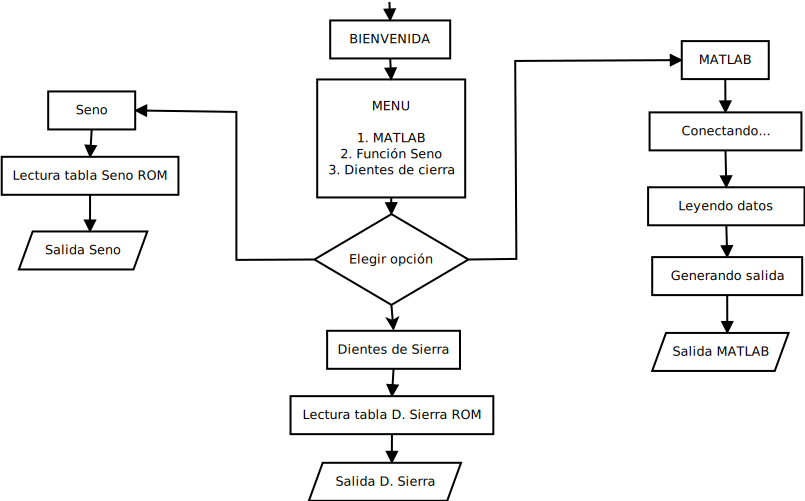
\includegraphics[width=1.0\textwidth]{images/flujo_menu_informe_v1.png}
  \caption{Diagrama de flujo del menú principal.}
  \label{fig:Diagrama de flujo}
\end{figure}

\section{Plan de trabajo}
\label{sec:plan_trabajo}
Fusce vitae accumsan ipsum. Pellentesque mauris leo, iaculis vitae orci in, tristique lobortis massa. Proin vitae varius dui. Sed aliquet convallis ornare. Ut enim justo, molestie non libero vitae, gravida sodales sem. Duis laoreet molestie tempus. Nulla vestibulum tristique nibh, consectetur convallis quam. Duis sollicitudin a dui eu iaculis. Proin pretium pharetra libero sed rutrum. Nunc mattis justo at justo volutpat luctus. Donec id eros ultrices, hendrerit dolor a, luctus metus. Mauris mi purus, congue at pulvinar a, sagittis in neque. 

\section{Listado de componentes y costos estimados}
\label{sec:componentes}

\begin{table}[H]
  \centering
  \begin{tabular}{ll}
    \toprule
    Componente & Costo estimado \\
    \midrule
    Microprocesador ATMega328p & \$ 110 \\
    Placa experimental & \$ ?? \\
    Soporte & \$ ?? \\
    Placa USB a Serie & $\approx$ \$ 120 \\
	Parlante & \$ ?? \\
    \midrule
    Total & \$ ?? \\
    \bottomrule
  \end{tabular}
  \caption{Costos estimados para la realización del proyecto.}
  \label{table:costos}
\end{table}

\section{Factores críticos de éxito}
\label{sec:fact_exito}

Es importante analizar cuáles son los riesgos potenciales más importantes que podrían dificultar la realización del proyecto. Una vez identificados, conviene hacerles un seguimiento cercano para evitar contratiempos.

- Desarrollo de inferfaz entre


% --------------------------------------------------
% Bibliografías
%\bibliography{biblio}{}
%\bibliographystyle{plain}
%\clearpage
% --------------------------------------------------
% Fin del informee
\end{document}
